\chapter{Environment}
Um die Forschungsfragen dieser Thesis zu beantworten, ist ein Environment nötig, welches auf minimale Weise Prozesse in einem Lager abbildet. Dabei soll das Environment so aufgebaut werden, dass ein Agent lernen muss, möglichst wenige Artikel am Lager zu halten, damit Kosten eingespart werden. Des Weiteren müssen wiederum genügend Artikel gelagert sein, sodass keine Lieferfrist vergeht und somit ein Auftrag storniert wird. Dieses Environment soll dabei möglichst erweiterbar aufgebaut werden und dem gängigen Standard von Reinforcement Learning Environments entsprechen. Dadurch wird sichergestellt, dass ohne grossen Aufwand verschiedene Algorithmen überprüft werden können.
\section{OpenAI Gym}
OpenAI, ein Unternehmen, welches sich mit der Erforschung von künstlicher Intelligenz beschäftigt, hat mit Gym \cite{gym} einen Standard für Reinforcement Learning geschaffen. Dabei war es ihr Ziel, eine Library an Environments zur Verfügung zu stellen, um Algorithmen einfacher über verschiedene Situationen zu benchmarken. Hierzu wurde darauf geachtet, dass das Aufsetzen eines Environments ohne grossen Aufwand möglich ist und somit auch die Reproduzierbarkeit veröffentlichter Forschung erleichtert wird.
\subsection{Gym-Methoden}
OpenAI Gym sollte folgende Methoden umfassen:
\begin{itemize}
    \item \textbf{step():} Diese Methode startet einen Zeitschritt im Environment, wobei die auszuführende Action übergeben wird. Der Rückgabe-Wert dieser Funktion enthält immer eine Observation vom Typ «object», ein Reward vom Typ «float», ein Flag vom Typ «boolean», welches bestimmt, ob die aktuelle Sequenz in einem Terminalstatus angekommen ist, sowie zusätzliche Debug-Informationen vom Typ «dict», welche für den Agent nicht sichtbar sein sollten. 
\item \textbf{render():} Diese optionale Methode ermöglicht es, mit dem Gym-integrierten Viewer ein Frame vom Environment zu rendern.
\item \textbf{reset():} Diese Methode setzt den aktuellen Status im Environment auf den Start zurück. Dabei wird hier auch eine erste Observation zurückgegeben. Reset wird im Normalfall zu Beginn und nach dem «\emph{done}»-Flag nach jeder Sequenz ausgeführt.

\end{itemize}








\subsection{Gym-Attribute}
Folgende Attribute müssen im Gym enthalten sein:
\begin{itemize}
    \item \textbf{observation\_space:} Dieses Attribut widerspiegelt den observierbaren State-Space. Dabei kann es ein Objekt sein, welches dasselbe Format hat wie die Observationen aus den reset()- und step()-Methoden oder eine Instanz der Klasse Space, welche von OpenAI zur Verfügung gestellt wird.
    \item \textbf{action\_space:} Dieses Attribut kann ein Array von möglichen Actions sein oder auch eine Instanz der Klasse Space.
\end{itemize}


\section{WarehouseEnv}
\label{sec:warehouse}
Beim erstellten «WarehouseEnv» handelt es sich um ein Environment, welches einen terminalen State hat. Jede Episode hat genau 100 Zeitschritte, sogenannte Steps. 

\begin{figure}[ht]
  \centering
  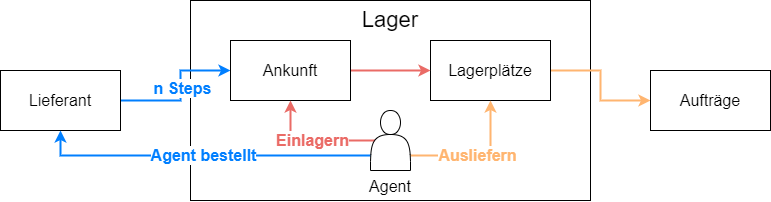
\includegraphics[width=\textwidth]{img/warehouse-env.png}
  \caption{WarehouseEnv}
    \label{fig:warehouse-env}
\end{figure} 

\newpage
\subsection{Environment-Step}
In jedem Step wird zuerst das Environment aktualisiert. Dabei wird überprüft, ob Aufträge storniert wurden und ob eine Bestellung im Wareneingang angekommen ist. Die Rewards dieser beiden Überprüfungen sowie ein Reward für die Lagerkosten werden nun vorgemerkt. Anschliessend findet die eigentliche Action statt; diese wird im Environment durchgeführt. Der Reward, welcher sich aus dem direkten Reward der Action sowie dem Reward der Aktualisierung ergibt, wird berechnet. Der Agent erhält nun eine Observation aus dem State und den Reward des durchgeführten Steps. \smallskip

\noindent\textbf{Lagerkosten}
\begin{table}[H]%
\begin{tabularx}{\textwidth} { 
  | >{\raggedright\arraybackslash}l 
  | >{\raggedright\arraybackslash}X | }
 \hline
 Reward &Dieser Reward wird vor jeder Aktion verteilt. Er ist abhängig vom genutzten Lagerplatz und soll somit Lagerkosten simulieren.\\
        &\textbf{-10 * Anzahl benutzter Lagerplätze}\\
\hline
\end{tabularx}
\caption{Lagerkosten}
\end{table}%

\noindent\textbf{Stornierter Auftrag}
\begin{table}[H]%
\begin{tabularx}{\textwidth} { 
  | >{\raggedright\arraybackslash}l 
  | >{\raggedright\arraybackslash}X | }
 \hline
 Reward &Dieser Reward wird vor jeder Aktion verteilt. Wird ein Auftrag storniert, so wird ein Reward von \textbf{-50} hinzugefügt.\\
\hline
\end{tabularx}
\caption{Stornierter Auftrag}
\end{table}%
\noindent\textbf{Bestellungseingang}
\begin{table}[ht]%
\begin{tabularx}{\textwidth} { 
  | >{\raggedright\arraybackslash}l 
  | >{\raggedright\arraybackslash}X | }
 \hline
 Reward	&Der Reward ist davon abhängig, ob im Wareneingang ein Platz frei ist.\\
&Artikel angekommen: \textbf{0}\\
&Artikel verworfen: \textbf{-25}\\
\hline
\end{tabularx}
\caption{Bestellungseingang}
\end{table}%

\newpage
\subsection{State-Space}
\label{sec:state-space}
Der State-Space besteht aus sämtlichen Entitäten und deren möglichen Zuständen. Die Anzahl der Entitäten sind jeweils Konstanten, welche im Environment festgelegt werden.
\noindent\textbf{Lagerplätze}
\begin{table}[H]%
\begin{tabularx}{\textwidth} { 
  | >{\raggedright\arraybackslash}l 
  | >{\raggedright\arraybackslash}X 
  | >{\raggedright\arraybackslash}l
  | >{\raggedright\arraybackslash}l|}
 \hline
  Anzahl &Anzahl der möglichen Lagerplätze &INT (const) &3\\
\hline
 Artikel &Pro Lagerplatz kann genau ein Artikel gelagert werden. &Artikel &Instanz\\
 \hline
\end{tabularx}
\caption{Lagerplätze}
\end{table}%
\noindent\textbf{Artikel}
\begin{table}[H]%
\smallskip
\begin{tabularx}{\textwidth} { 
  | >{\raggedright\arraybackslash}l 
  | >{\raggedright\arraybackslash}X 
  | >{\raggedright\arraybackslash}l
  | >{\raggedright\arraybackslash}l|}
 \hline
  Anzahl &Anzahl der möglichen Artikel &INT (const) &1\\
\hline
 Häufigkeit &Die Häufigkeit definiert, mit welcher Wahrscheinlichkeit ein Artikel bestellt wird. &FLOAT &[0-1]\\
 \hline
\end{tabularx}
\caption{Artikel}
\end{table}%

\noindent\textbf{Aufträge}\\
Sofern nicht die maximale Anzahl an Aufträgen ansteht, wird nach jedem vierten Step ein neuer Auftrag generiert. Dabei wird der Artikel nach der Artikelhäufigkeit gewählt. Ein Auftrag hat ausserdem eine Frist von 5 Steps. Wurde der Auftrag nicht ausgeliefert und somit abgeschlossen, so wird dieser vom Auftraggeber storniert.
\begin{table}[H]%
\begin{tabularx}{\textwidth} { 
  | >{\raggedright\arraybackslash}l 
  | >{\raggedright\arraybackslash}X 
  | >{\raggedright\arraybackslash}l
  | >{\raggedright\arraybackslash}l|}
 \hline
  Anzahl &Maximale Anzahl anstehender Aufträge &INT (const) &2\\
\hline
 Artikel &Jeder Auftrag enthält genau einen Artikel.  &Artikel &Instanz\\
 \hline
\end{tabularx}
\caption{Aufträge}
\end{table}%

\noindent\textbf{Wareneingang}\\
Die Artikel, die beim Hersteller bestellt wurden, erscheinen nach der Lieferzeit von zwei Steps im Wareneingang. 
\begin{table}[H]%
\begin{tabularx}{\textwidth} { 
  | >{\raggedright\arraybackslash}l 
  | >{\raggedright\arraybackslash}X 
  | >{\raggedright\arraybackslash}l
  | >{\raggedright\arraybackslash}l|}
 \hline
  Anzahl &Anzahl der Plätze im Wareneingang &INT (const) &2\\
\hline
 Artikel &Jeder Platz im Wareneingang kann genau einen Artikel enthalten.   &Artikel &Instanz\\
 \hline
\end{tabularx}
\caption{Wareneingang}
\end{table}%


\noindent\textbf{Bestellungen}\\
Gibt der Agent eine Bestellung auf, so ist diese hier ersichtlich, bis der Artikel im Wareneingang eingetroffen ist. 
\begin{table}[H]%
\begin{tabularx}{\textwidth} { 
  | >{\raggedright\arraybackslash}l 
  | >{\raggedright\arraybackslash}X 
  | >{\raggedright\arraybackslash}l
  | >{\raggedright\arraybackslash}l|}
 \hline
  Anzahl &Anzahl der gleichzeitigen Bestellungen &INT (const) &2\\
\hline
 Artikel &Jede Bestellung enthält genau einen Artikel.    &Artikel &Instanz\\
 \hline
\end{tabularx}
\caption{Bestellungen}
\end{table}%

\noindent Eine Observation, welche dem Agent nach jedem Step zur Verfügung steht, besteht aus folgenden Teilen.
\begin{table}[H]%
\begin{tabularx}{\textwidth} { 
  | >{\raggedright\arraybackslash}X 
  | >{\raggedright\arraybackslash}l 
  | >{\raggedright\arraybackslash}l
  | >{\raggedright\arraybackslash}l
  | >{\raggedright\arraybackslash}l|}
 \hline
  State-Teil &Lagerplätze &Aufträge &Wareneingang &Bestellungen\\
\hline
 Möglicher Zustand &[0,0,0] &[0,0] &[0,0] &[0,0] \\
 \hline
\end{tabularx}
\caption{Observation}
\end{table}%
\noindent Dabei kann in jedem Element der State 0 für keinen Artikel, 1 für Artikel 1 und 2 für Artikel 2 angenommen werden.

\newpage
\subsection{Action-Space}
Der Action-Space definiert die möglichen Aktionen, die der Agent ausführen kann: \\
\noindent\textbf{Lagern}
\begin{table}[H]%
\begin{tabularx}{\textwidth} { 
  | >{\raggedright\arraybackslash}l 
  | >{\raggedright\arraybackslash}X|}
 \hline
  Ablauf &Nimmt einen Artikel aus dem Wareneingang und platziert diesen im Lager\\
\hline
 Reward &Der Reward ist abhängig vom Erfolg des Einlagerns:\\
&Erfolgreiches einlagern: \textbf{0}\\
&Besetzter Platz: \textbf{-10}\\
 \hline
\end{tabularx}
\caption{Lagern}
\end{table}%

\noindent\textbf{Ausliefern}
\begin{table}[H]%
\begin{tabularx}{\textwidth} { 
  | >{\raggedright\arraybackslash}l 
  | >{\raggedright\arraybackslash}X|}
 \hline
  Ablauf &Nimmt einen Artikel aus dem Lager und schliesst damit den gewählten Auftrag ab\\
\hline
 Reward &Der Reward ist abhängig vom Erfolg der Aktion:\\
&Richtiger Artikel abgegeben: \textbf{100}\\
&Falscher Artikel abgegeben: \textbf{-100}\\
 \hline
\end{tabularx}
\caption{Ausliefern}
\end{table}%

\noindent\textbf{Bestellen}
\begin{table}[H]%
\begin{tabularx}{\textwidth} { 
  | >{\raggedright\arraybackslash}l 
  | >{\raggedright\arraybackslash}X|}
 \hline
  Ablauf &Bestellt einen Artikel beim Lieferanten; der Artikel wird nach zwei weiteren Actions im Wareneingang ankommen. Sind im Wareneingang bereits alle Plätze besetzt, so wird der Artikel verworfen.\\
\hline
 Reward &Hier entsteht kein direkter Reward, der Reward wird bei der Ankunft berechnet.\\
 \hline
\end{tabularx}
\caption{Bestellen}
\end{table}%

\noindent\textbf{Warten}
\begin{table}[H]%
\begin{tabularx}{\textwidth} { 
  | >{\raggedright\arraybackslash}l 
  | >{\raggedright\arraybackslash}X|}
 \hline
  Ablauf &Diese Action ist ein Platzhalter; es wird im Environment der Step durchgeführt, jedoch keine Action.\\
\hline
 Reward &Der Reward dieser Action ist immer \textbf{0}.\\
 \hline
\end{tabularx}
\caption{Warten}
\end{table}%


\subsection{Orakel}
Um die Komplexität zu verringern, werden zwei Orakel verwendet. Es handelt sich hierbei um Entscheidungen, welche nach einfachen Bedingungen optimal gelöst werden können. 
\textbf{Lagerplatz wählen:}\\ Dieses Orakel gibt dem Agent einen möglichen Lagerplatz. Damit wird ausgeschlossen, dass ein bereits besetzter Platz gewählt wird.\\
\textbf{Artikel für die Lieferung wählen:}\\ Dieses Orakel gibt dem Agent einen Artikel an, welcher geliefert werden kann. Damit kann ausgeschlossen werden, dass ein falscher Artikel ausgeliefert wird. Es wird automatisch der Auftrag gewählt, welcher am längsten offen ist.



\section {Heuristik}
Um die durch Reinforcement Learning erlernte Strategie zu vergleichen, wird eine Heuristik definiert. Ein Agent wird nach dieser Anleitung seine Actions wählen:\\
\textbf{Priorität 1 – Ausliefern:}\\
Sofern eine Bestellung ansteht und der entsprechende Artikel im Lager ist, wird dieser Artikel ausgeliefert. Dadurch sollen die Lagerkosten geringgehalten und das Ablaufen einer Bestellung vermieden werden.\\
\textbf{Priorität 2 – Einlagern:}\\
Da im Lagereingang nur begrenzt Platz vorhanden ist, sollen Artikel möglichst schnell eingelagert werden.\\
\textbf{Priorität 3 – Bestellen:}\\
Es wird ein Artikel bestellt, sofern nicht bereits einer am Lager ist oder bestellt wurde.\\
\textbf{Priorität 4 – Warten:}\\
In diesem Fall macht der Agent nichts; es soll vermieden werden, dass unnötige Lagerplätze besetzt werden.


\section{Komplexität des Problems}
Um die für Forschungsfrage 2 relevante Komplexität des Problems zu erhöhen, werden nicht die Orakel entfernt, denn diese haben nur simple Entscheidungen zu fällen. Eine sinnvollere Komplexitätssteigerung wird durch das Hinzufügen eines weiteren Artikels erreicht. Dieser Artikel erhöht damit den State und zwingt den Agent zu bestimmen, welcher Artikel bestellt werden soll.